\chapter{Preliminaries: Set theory and categories}
\section{Naive set theory}
\problem{
    Locate a discussion of Russell's paradox, and understand it.
}{
    Recall that, in naive set theory, any collection of objects satisfying some properties can be called a set. Russel's paradox can be illustrated as follows:

    Let $R$ be the set of all sets that do not contain themselves. Then, if $R \notin R$, then by definition it must be the case that $R \in R$. Similarly, if $R \in R$ then it must be the case that $R \notin R$.

    This is the reason why we need the axiomatic set theory instead of the naive set theory.
}

\problem{
    $\vartriangleright$ Prove that if $\sim$ is an equivalence relation on a set $S$, then the corresponding family $\mathscr{P}_\sim$ defined in \S 1.5 is indeed a partition of $S$; that is, its elements are nonempty, disjoint, and their union is $S$. $\left[ \text{\S1.5} \right]$
}{
    Let $S$ be a set with an equivalence relation $\sim$. Consider the family of equivalence classes with respect to $\sim$ over $S$:
    $$\mathscr{P}_\sim = \{ \left[ a \right]_\sim \mid a \in S \}$$

    Let $\left[ a \right]_\sim \in \mathscr{P}_\sim$. Then by reflexivity of $\sim$, we have $a \sim a$ and thus $\left[ a \right]_\sim$ is nonempty. 

    Now, take any two elements $\left[ a \right]_\sim$ and $\left[ b \right]_\sim$ of $\mathscr{P}_\sim$. If $\left[ a \right]_\sim \cap \left[ b \right]_\sim$ is nonempty, then we can take an element $c \in \left[ a \right]_\sim \cap \left[ b \right]_\sim$. By definition, we get $c \sim a$ and $c \sim b$. By symmetricity of $\sim$, we get $a \sim c$ and so $a \sim b$ by transitivity of $\sim$. This means that $a \in \left[ b \right]_\sim$, and by transitivity of $\sim$, we can conclude that $\left[ a \right]_\sim \subseteq \left[ b \right]_\sim$.

    In the same way, we also can conclude that $\left[ b \right]_\sim \subseteq \left[ a \right]_\sim$ when $\left[ a \right]_\sim \cap \left[ b \right]_\sim$ is nonempty, and hence $\left[ a \right]_\sim = \left[ b \right]_\sim$ if $\left[ a \right]_\sim \cap \left[ b \right]_\sim$ is nonempty. In the other words, the elements of $\mathscr{P}_\sim$ are disjoint.
    
    Finally, for any $a \in S$, $a \in \left[ a \right]_\sim$, and thus $S \subseteq \bigcup \mathscr{P}_\sim$, obviously. Also, since $\sim$ is a relation on the set $S$, $\bigcup \mathscr{P}_\sim \subseteq S$, indeed.

    Therefore, $\mathscr{P}_\sim$ is a partition of $S$.
}

\problem{
    $\vartriangleright$ Given a partition $\mathscr{P}$ on a set $S$, show how to define an equivalence relation $\sim$ on $S$ such that $\mathscr{P}$ is the corresponding partition. $\left[ \text{\S1.5} \right]$
}{
    Let $S$ be a set with a partition $\mathscr{P}$. Consider a relation $\sim$ on $S$ as:
    $$a \sim b \iff \exists P \in \mathscr{P} \st a,b \in P.$$

    Then, it is quite obvious that $\sim$ is an equivalence relation.
}

\problem{
    How many different equivalence relations may be defined on the set $\{ 1,2,3 \}$?
}{
    Since there is a correspondence between equivalence relations and partitions, the number of equivalence relations is the same with the number of partitions. Since there are 5 different partitions of the set $\{ 1,2,3 \}$, there are 5 different equivalence relations can be defined on the set $\{ 1,2,3 \}$.
}

\problem{
    Give an example of a relation that is reflexive and symmetric but not transitive. What happens if you attempt to use this relation to define a partition on the set?
}{
    For $a,b \in \RR$, define $a \mathrel{\mathcal{R}} b$ to be true if and only if $\abs{a-b} \leq 1$. Then, it is obvious that $\mathrel{\mathcal{R}}$ is reflexive and symmetric. However, since $0 \not\mathrel{\mathcal{R}} 2$ even though $0 \mathrel{\mathcal{R}} 1$ and $1 \mathrel{\mathcal{R}} 2$, $\mathrel{\mathcal{R}}$ is not transitive. The corresponding family $\mathscr{P}_{\mathrel{\mathcal{R}}}$, defined as in \S 1.5, is not a partition of $\RR$, indeed  because the elements of $\mathscr{P}_{\mathrel{\mathcal{R}}}$ are not disjoint.
}

\problem{
    $\vartriangleright$ Define a relation $\sim$ on the set $\RR$ of real numbers by setting $a \sim b \iff b-a \in \ZZ$.  Prove that this is an equivalence relation, and find a `compelling' description for $\RR / \sim$. Do the same for the relation $\approx$ on the plane $\RR \times \RR$ defined by declaring  $\left( a_1,a_2 \right) \approx \left( b_1,b_2 \right) \iff b_1 - a_1 \in \ZZ$ and $b_2 - a_2 \in \ZZ$.  $\left[ \text{\S{}II.8.1, II.8.10} \right]$
}{
    Since $0 \in \ZZ$, $-n \in \ZZ$ for any $n \in \ZZ$, and $n+m \in \ZZ$ for any $n,m \in \ZZ$, the given relation $\sim$ on $\RR$ is an equivalence relation. Moreover, $\RR / \sim$ can be considered as $\lcint{0}{1}$ with operation on modulo 1. (It can be considered as $S^1$.)

    Now define a relation $\approx$ on $\RR^2$ by setting $\left( a_1,a_2 \right) \approx \left( b_1,b_2 \right) \iff a_1 - a_2 \in \ZZ$ and $b_1 - b_2 \in \ZZ$. Then by the similar way with the above, the relation $\approx$ on $\RR^2$ is an equivalence relation. Additionally, $\RR^2 / \approx$ is isomorphic to $\lcint{0}{1} \times \lcint{0}{1}$ with operation on modulo 1. (It can be considered as $T^2$.)
}

\newpage
\section{Functions between Sets}

\problem{
    $\vartriangleright$ How many different bijections are there between a set $S$ with $n$ elements and itself?
}{
    The answer is $n!$, obviously.
}

\problem{
    $\vartriangleright$ Prove statement (2) in Proposition 2.1. You may assume that given a family of disjoint nonempty subsets of a set, there is a way to choose one element in each member of the family. $\left[ \text{\S2.5, V.3.3} \right]$
}{
    \begin{itemize}[leftmargin=12mm]
        \item[]
        \item[($\implies$)] Let's say that $f : A \to B$ has a right-inverse $g : B \to A$. Then since $f \circ g = \id_B$, $(f \circ g)(B) = B$, clearly.
        
        By the fact that $(f \circ g)(B) = f(g(B)) \subseteq f(A) \subseteq B$, it is immediately shown that $f(A) = B$, i.e., $f$ is surjective.
        
        \item[($\impliedby$)] Let's say that $f : A \to B$ is surjective. Then $f^{-1}(b) = \{ a \in A \mid f(a) = b \}$ is nonempty for any $b$ and also $\{ f^{-1}(b) \mid b \in B \}$ is a partition of $A$, clearly.

        Thus, by the axiom of choice---the given statement is the stronger version of the axiom of choice, we can take a function $g : B \to A$ such that $g(b) \in f^{-1}(b)$ for any $b \in B$.

        Then $(f \circ g)(b) = b$ for any $b \in B$ and $f$ therefore has a right-inverse $g : B \to A$.
    \end{itemize}
}

\problem{
    Prove that the inverse of a bijection is a bijection and that the composition of two bijection is a bijection.
}{
    By Proposition 2.1, it is clear that the inverse of a bijection is also a bijection and that the composition of two bijections is also a bijection.
}

\problem{
    $\vartriangleright$ Prove that `isomorphism' is an equivalence relation (on any set of sets). \(\left[ \text{\S4.1} \right]\)
}{
    Let $U$ be a set of sets and define a relation $\sim$ on $U$ by setting $S \sim T \iff S$ is isomorphic to $T$.
    
    Then it is clear that $S \sim S$ for any $S \in U$ since $\id_S$ is a bijection.

    Moreover, by the result of the Exercise 2.3, the relation $\sim$ on $U$ is symmetric and transitive.
    
    Therefore, the relation $\sim$ on $U$ is an equivalence relation.
}

\problem{
    $\vartriangleright$ Formulate a notion of \emph{epimorphism}, in the style of the notion of \emph{monomorphism} seen in \S2.6, and prove a result analogous to Proposition 2.3, for epimorphism and surjections. \(\left[ \S2.6, \S4.2 \right]\)
}{
    A function $f : A \to B$ is an epimorphism if the following holds:
    \begin{center}
        for all sets $Z$ and all functions $\alpha', \alpha'' : B \to Z$, $\alpha' \circ f = \alpha'' \circ f \implies \alpha' = \alpha''$.
    \end{center}

    Now claim that a function $f : A \to B$ is an epimorphism if and only if it is a surjection. The below is the proof of that:

    \begin{itemize}[leftmargin=12mm]
        \item[($\implies$)] Let's say that $f : A \to B$ is an epimorphism and suppose that $f$ is not surjective. Then $B \setminus f(A)$ is nonempty and so there exists $b \in B \setminus f(A)$. Now say that $\alpha' = \id_B$ and $\alpha'' : B \to B$ is defined by $x \mapsto \begin{cases}x & \mbox{if } x \neq b \\ b' & \mbox{if } x=b\end{cases}$ where $b'$ is an element of $f(A)$.

        Then it is obvious that $\alpha' \circ f = \alpha'' \circ f$ and this contradicts the fact that $f$ is an epimorphism.

        Therefore, $f$ has to be surjective.
        
        \item[($\impliedby$)] Let's say that $f : A \to B$ is a surjection and $\alpha' \circ f = \alpha'' \circ f$ for some $\alpha', \alpha'' : B \to Z$ for a fixed set $Z$.
        
        Then since $f(A) = B$, $\alpha' \circ f = \alpha'' \circ f$ implies that $\alpha'(b) = \alpha''(b)$ for any $b \in B$, and this clearly implies that $\alpha' = \alpha''$.

        Therefore, $f$ is an epimorphism.
    \end{itemize}
}

\problem{
    With notation as in Example 2.4, explain how any function $f : A \to B$ determines a section of $\pi_A$.
}{
    Define $\gamma_f : A \to A \times B$ as $a \mapsto \left( a,f(a) \right)$. Then $\left( \pi_A \circ \gamma_f \right)(a) = \pi_A \left( a,f(a) \right) = a$ and thus makes $\gamma_f$ be a right-inverse of $\pi_A$, i.e., $\gamma_f$ is a section of $\pi_A$.
}

\problem{
    Let $f : A \to B$ be any function. Prove that the graph $\Gamma_f$ of $f$ is isomorphic to $A$.
}{
    Let $\varphi : A \to \Gamma_f$ be a function defined as $\varphi : a \mapsto \left( a,f(a) \right)$.

    Then it is obvious that $\varphi$ is a bijection by the definition of a graph of a function. Therefore, $A$ and $\Gamma_f$ are isomorphic to each other.
}

\problem{
    Describe as explicitly as you can all terms in the canonical decomposition (cf. \S2.8) of the function $\RR \to \CC$ defined by $r \mapsto e^{2\pi ir}$. (This exercise matches one assigned previously. Which one?)
}{
    Let $f : \RR \to \CC$ be defined by $r \mapsto e^{2\pi ir}$.

    Now let's say that $\pi : \RR \twoheadrightarrow \lcint{0}{1}$, $\tilde{f} : \lcint{0}{1} \twoheadhookrightarrow \{ z \in \CC \mid \abs{z} = 1 \}$, and $\iota : \{ z \in \CC \mid \abs{z} = 1 \} \to \CC$ are defined as:
    $$\begin{array}{l}
        \pi : r \mapsto r \bmod 1 \\
        \tilde{f} : r \mapsto e^{2\pi ir} \\
        \iota : z \mapsto z.
    \end{array}$$

    Then, $f = \iota \circ \tilde{f} \circ \pi$ is the canonical decomposition of $f$. Also, this exercise matches Exercise 1.6.
}

\problem{
    $\vartriangleright$ Show that if $A' \cong A''$ and $B' \cong B''$, and further $A' \cap B' = \emptyset$ and $A'' \cap B'' = \emptyset$, then $A' \cup B' \cong A'' \cup B''$. Conclude that the operation $A \sqcup B$ (as described in \S1.4) is well-defined \emph{up to isomorphism} (cf. \S2.9). $\left[ \text{\S2.9, 5.7} \right]$
}{
    Since $A' \cap B' = \emptyset$, if $x \in A' \cup B'$, only one of the following holds:
    \begin{enumerate}[label=\alph*)]
        \item $x \in A'$
        \item $x \in B'$
    \end{enumerate}
    Furthermore, $A''$ and $B''$ also satisfy the same property.

    Now let $\alpha : A' \to A''$ and $\beta : B' \to B''$ be bijections. Then we can define a function $\varphi : A' \cup B' \to A'' \cup B''$ as $x \mapsto \begin{cases} \alpha(x) & \mbox{if } x \in A' \\ \beta(x) & \mbox{if } x \in B'. \end{cases}$

    By the facts proved above, $\varphi$ is obviously a bijection. Therefore, $A' \cong A''$, $B' \cong B''$, $A' \cap B' = \emptyset$, and $A'' \cap B'' = \emptyset$ imply that $A' \cup B' \cong A'' \cup B''$ and, hence, the operation $A \sqcup B$ is well-defined up to isomorphism.
}

\problem{
    $\vartriangleright$ Show that if $A$ and $B$ are finite sets, $\abs{B^A} = \abs{B}^{\abs{A}}$. \(\left[ \text{\S2.1, 2.11, \S II.4.1}\right]\)
}{
    Since $A^B$ is the set of the functions to $A$ from $B$, $\abs{B^A}$ is the number of functions from $A$ to $B$. For each element of $A$, there exist $\abs{B}$ possible function values and thus $\abs{B^A} = \abs{B}^{\abs{A}}$.
}

\problem{
    $\vartriangleright$ In view of Exercise 2.10, it is not unreasonable to use $2^A$ to denote the set of functions from an arbitrary set $A$ to set with 2 elements (say $\{ 1,2 \}$). Prove that there is a bijection between $2^A$ and the \emph{power set} of $A$ (cf. \S1.2). \(\left[ \S1.2, III.2.3 \right]\)
}{
    Define $f : 2^A \to \mathscr{P}(A)$ as $\varphi \mapsto \{ a \in A \mid \varphi(a) = 1 \}$. Then it is quite obvious that $f$ is a bijection. Therefore, $2^A \cong \mathscr{P}(A)$.
}

\newpage
\section{Categories}
\problem{
    $\vartriangleright$ Let $\cat{C}$ be a category. Consider a structure $\op{\cat{C}}$ with
    \begin{itemize}[label=$\bullet$]
        \item $\Obj{\op{\cat{C}}} := \Obj{\cat{C}}$
        \item for $A$, $B$ objects of $\op{\cat{C}}$ (hence objects of $\cat{C}$), $\Hom{\op{\cat{C}}}{A}{B} := \Hom{\cat{C}}{B}{A}$.
    \end{itemize}
    Show how to make this into a category (that is, define composition of morphisms in $\op{\cat{C}}$ and verify the properties listed in \S3.1).
}{
    For any objects $A,B,C$ of the category $\op{\cat{C}}$, let $gf \in \Hom{\op{\cat{C}}}{A}{C}$ be $fg \in \Hom{\cat{C}}{C}{A}$ where $f \in \Hom{\op{\cat{C}}}{A}{B}$ and $g \in \Hom{\op{\cat{C}}}{B}{C}$, and also $fg \in \Hom{\cat{C}}{C}{A}$ are already defined.

    Then by the associativity of the composition in the category $\cat{C}$, the composition in the category $\op{\cat{C}}$ is also associative. Moreover, the identity $\one_A$ on an object $A$ in the category $\cat{C}$ is also identity on an object $A$ in the category $\op{\cat{C}}$.

    Therefore, $\op{\cat{C}}$ is also a category if $\cat{C}$ is a category.
}

\problem{
    If $A$ is a finite set, how large is $\End{\Set}{A}$?
}{
    Since $\End{\Set}{A} = A^A$ and $A$ is finite, $\abs{\End{\Set}{A}} = \abs{A}^{\abs{A}}$ by the result of \ref{prob:2.10}.
}

\problem{
    $\vartriangleright$ Formulate precisely what it means to say that $\one_a$ is an identity with respect to composition in Example 3.3, and prove this assertion. \(\left[ \text{\S3.2} \right]\)
}{
    For any objects $b$ of the category in Example 3.3, and for any morphisms $f \in \Hom{}{a}{b}$ and $g \in \Hom{}{b}{a}$, $f\one_a = f$ and $\one_a g = g$.

    To prove this statement, let's think about the definition of $\Hom{}{a}{b}$ in Example 3.3, and the definition of the composition in Example 3.3. By the definition, $f \in \Hom{}{a}{b}$ means that $a \sim b$ and $f = (a,b)$. Also, $f\one_a = (a,b)(a,a) = (a,b) = f$ by the definition.

    Similarly, we can show that $\one_a g = g$ for any $g \in \Hom{}{b}{a}$.

    Therefore, $\one_a$ is an identity with respect to composition in Example 3.3.
}

\problem{
    Can we define a category in the style of Example 3.3 using the relation $<$ on the set $\ZZ$?
}{
    Since the relation $<$ is not reflexive, if we define a category-like structure in the style of Example 3.3, there is no identity. Hence, we cannot define a category in the style of Example 3.3 using the relation $<$ on the set $\ZZ$.
}

\problem{
    $\vartriangleright$ Explain in what sense Example 3.4 is an instance of the categories considered in Example 3.3. \(\left[ \text{\S3.2} \right]\)
}{
    Since $\subseteq$ is reflexive and transitive, $\subseteq$ on $\mathscr{P}(S)$ makes a category in the style of Example 3.3.

    We can observe that the category in Example 3.4 and the category we just made in the style of Example 3.3 are actually the same.
}

\problem{
    $\vartriangleright$ (Assuming some familiarity with linear algebra.) Define a category $\cat{V}$ by taking $\Obj{\cat{V}} = \NN$ and letting $\Hom{\cat{V}}{n}{m} = \text{the set of } m \times n$ matrices with real entries, for all $n,m \in \NN$. (We will leave the reader the task of making sense of a matrix with 0 rows or columns.) Use product of matrices to define composition. Does this category `feel' familiar? \(\left[ \text{\S VI.2.1, \S VIII.1.3} \right]\)
}{
    $n \times m$ real-entry-matrices can be considered as a linear transform from $\RR^n$ to $\RR^m$. Hence, we can consider the category $\cat{V}$ as a category whose objects are $\RR^n$ spaces and morphisms are linear transform between them.
}

\problembr{
    $\vartriangleright$ Define carefully objects and morphisms in Example 3.7, and draw the diagram corresponding to composition. \(\left[ \text{\S3.2} \right]\)
}{
    Let $\cat{C}$ be a category and $A$ be an object of $\cat{C}$. We are going to define a category $\cat{C}^A$ whose objects are certain morphisms in $\cat{C}$ and whose morphisms are certain diagrams of $\cat{C}$.

    Let $\Obj{\cat{C}^A}$ be the collection of all morphisms from $A$ to any objects of $\cat{C}$; thus, an object of $\cat{C}^A$ is a morphism $f \in \Hom{\cat{C}}{A}{Z}$ for some objects $Z$ of $\cat{C}$. Now let $f_1,f_2$ be objects of $\cat{C}^A$, that is, two arrows
    \begin{cd} 
        A \ar[d, "f_1"] \& A \ar[d, "f_2"] \\
        Z_1 \& Z_2
    \end{cd}
    in $\cat{C}$. Morphisms $f_1 \to f_2$ are defined to be commutative diagrams
    \[\begin{tikzcd}[column sep=1.5em,ampersand replacement=\&]
        \& A \ar[dl, swap, "f_1"] \ar[dr, "f_2"] \\
        Z_1 \ar[rr, "\sigma"] \&\& Z_2
    \end{tikzcd}\]
    in the category $\cat{C}$.

    Now let's define the composition in $\cat{C}^A$. Let two morphisms $f_1 \to f_2$ and $f_2 \to f_3$ be given:
    \[\begin{tikzcd}[column sep=1.5em,ampersand replacement=\&]
        \& A \ar[dl, swap, "f_1"] \ar[dr, "f_2"] \&\&\& A \ar[dl, swap, "f_2"] \ar[dr, "f_3"] \\
        Z_1 \ar[rr, "\sigma"] \&\& Z_2 \& Z_2 \ar[rr, "\tau"] \&\& Z_3
    \end{tikzcd}\]
    Then the following diagram is also commutative so it is a morphism in $\cat{C}^A$:
    \[\begin{tikzcd}[column sep=1.5em,ampersand replacement=\&]
        \& A \ar[dl, swap, "f_1"] \ar[dr, "f_3"] \\
        Z_1 \ar[rr, "\tau\sigma"] \&\& Z_3
    \end{tikzcd}\]
    If we define the composition in the way mentioned above, the composition is associative, indeed.
    
    Moreover, there is an identity $\one_f : f \to f$. Look at the diagram below:
    \[\begin{tikzcd}[column sep=1.5em,ampersand replacement=\&]
        \& A \ar[dl, swap, "f"] \ar[dr, "f"] \\
        Z \ar[rr, "\one_Z"] \&\& Z
    \end{tikzcd}\]
    The diagram above is obviously commutative, so it is a morphism $f \to f$. Also, it is quite clear that the above diagram is an identity.

    Therefore, $\cat{C}^A$ is a category.
}

\problem{
    $\vartriangleright$ A \emph{subcategory} $\cat{C'}$ of a category $\cat{C}$ consists of a collection of objects of $\cat{C}$, with morphisms $\Hom{\cat{C'}}{A}{B} \subseteq \Hom{\cat{C}}{A}{B}$ for all objects $A$, $B$ in $\Obj{\cat{C'}}$, such that identities and compositions in $\cat{C}$ make $\cat{C'}$ into a category. A subcategory $\cat{C'}$ is \emph{full} if $\Hom{\cat{C'}}{A}{B} = \Hom{\cat{C}}{A}{B}$ for all $A,B$ in $\Obj{\cat{C'}}$. Construct a category of \emph{infinite sets} and explain how it may be viewed as a full subcategory of $\Set$. \(\left[ \text{4.4, \S VI.1.1, \S VIII.1.3 }\right]\)
}{
    Let $\cat{S}$ be a category which satisfies the following:
    \begin{itemize}[label=$\bullet$]
        \item $\Obj{\cat{S}}$ is the collection of the infinite sets.

        \item For any infinite sets $A,B \in \Obj{\cat{S}}$, $\Hom{\cat{S}}{A}{B}$ is the collection of all functions $A \to B$.
    \end{itemize}
    Then it is obvious that $\cat{S}$ is a full subcategory of $\Set$.
}

\problembr{
    $\vartriangleright$ An alternative to the notion of \emph{multiset} introduced in \S2.2 is obtained by considering sets endowed with equivalence relations; equivalent elements are taken to be multiple instances of elements `of the same kind'. Define a notion of morphism between such enhanced sets, obtaining a category $\MSet$ containing (a `copy' of) $\Set$ as a full subcategory. (There may be more than one reasonable way to do this! This is intentionally an open-ended exercise.) Which objects in $\MSet$ determine ordinary multisets as defined in \S2.2 and how? Spell out what a morphism of multisets would be from this point of view. (There are several natural notions of morphisms of multisets. Try to define morphisms in $\MSet$ so that the notion you obtain for ordinary multisets captures your intuitive understanding of these objects.) \(\left[ \text{\S2.2, \S3.2, 4.5} \right]\)
}{
    Before formalizing the concept of multisets, let's think about the concept of multisets in an informal way.

    The multisets are collections of elements may occur more than once; the occurences of a particular element in a multiset are indistinguishable. Moreover, the number of the occurences of a particular element in a multiset is a positive integer. To formalize this, we will use a concept of functions.

    Let $A$ be a set and $m : A \to \ZZ^+$ be a function where $\ZZ^+$ denotes the set of the positive integers. Then a 2-tuple $(A,m)$ is a multiset. From this point of view, $(A, x \mapsto 1 )$ is a `copy' of a set $A$.

    Now consider about morphisms between two multisets. The morphisms $(A,m_A) \to (B,m_B)$ are defined to be functions $A \to B$. Then an identity morphism $\one_{(A,m)}$ is the identity function $\id_A : A \to A : a \mapsto a$.

    The composition is defined as the composition of two functions, indeed.

    Then identity morphisms are identities with respect to composition, and the composition is associative.

    Therefore, $\MSet$ is a category if we define $\MSet$ in the way mentioned above, and the `copy' of $\Set$ is a full subcategory of $\MSet$.
}

\problem{
    Since the objects of a category $\cat{C}$ are not (necessarily interpreted as) sets, it is not clear how to make sense of notion of `subobject' in general, extrapolating the notion of subset. In some situations it \emph{does} make sense to talk about subobjects, and the subobjects of any given object $A$ in $\cat{C}$ are in one-to-one correspondence with the morphisms $A \to \Omega$ for a fixed, special object $\Omega$ of $\cat{C}$, called a \emph{subobject classifier}. Show that $\Set$ has a subobject classifier.
}{
    Since $2^A$ and $\mathscr{P}(A)$ are isomorphic to each other in the category $\Set$, we can choose the set $\{ 0,1 \}$ as the subobject classifier of the category $\Set$.
}

\problembr{
    $\vartriangleright$ Draw the relevant diagrams and define composition and identities for the category $\cat{C}^{A,B}$ mentioned in Example 3.9. Do the same for the category $\cat{C}^{\alpha, \beta}$ mentioned in Example 3.10. \(\left[ \text{\S5.5, 5.12} \right]\)
}{
    At this time, we start from a given category $\cat{C}$ and two objects $A,B$ of $\cat{C}$. We can define a new category $\cat{C}^{A,B}$ by essentially the same procedure that we used in order to define $\cat{C}^A$:
    \begin{itemize}[label=$\bullet$]
        \item $\Obj{\cat{C}^{A,B}}$ is the collection of the diagrams
        \[\begin{tikzcd}[row sep=0.8em,column sep=2em,ampersand replacement=\&]
            \&\& A \ar[dll, swap, "f"] \\
            Z \\
            \&\& B \ar[ull, "g"]
        \end{tikzcd}\]
        in $\cat{C}$;

        \item morphisms
        \[\begin{tikzcd}[row sep=0.8em,column sep=2em,ampersand replacement=\&]
            \&\& A \ar[dll, swap, "f_1"] \&\& \&\& A \ar[dll, swap, "f_2"] \\
            Z_1 \&\& \ar[rr] \&\& Z_2\\
            \&\& B \ar[ull, "g_1"] \&\& \&\& B \ar[ull, "g_2"]
        \end{tikzcd}\]
        are commutative diagrams:
        \[\begin{tikzcd}[row sep=0.8em,column sep=2em,ampersand replacement=\&]
            \&\&\& A \ar[dll, "f_2"] \ar[dlll, swap, bend right, "f_1"] \\
            Z_1 \& Z_2 \ar[l, swap, "\sigma"] \\
            \&\&\& B \ar[ull, swap, "g_2"] \ar[ulll, bend left, "g_1"]
        \end{tikzcd}\]
        in $\cat{C}$;

        \item composition of two morphisms
        \[\begin{array}{ll}
            \begin{tikzcd}[row sep=0.8em,column sep=2em,ampersand replacement=\&]
                \&\&\& A \ar[dll, "f_2"] \ar[dlll, swap, bend right, "f_1"] \\
                Z_1 \& Z_2 \ar[l, swap, "\sigma"] \\
                \&\&\& B \ar[ull, swap, "g_2"] \ar[ulll, bend left, "g_1"]
            \end{tikzcd}, &
            \begin{tikzcd}[row sep=0.8em,column sep=2em,ampersand replacement=\&]
                \&\&\& A \ar[dll, "f_3"] \ar[dlll, swap, bend right, "f_2"] \\
                Z_2 \& Z_3 \ar[l, swap, "\tau"] \\
                \&\&\& B \ar[ull, swap, "g_3"] \ar[ulll, bend left, "g_2"]
            \end{tikzcd}
        \end{array}\]
        is a commutative diagram
        \[\begin{tikzcd}[row sep=0.8em,column sep=2em,ampersand replacement=\&]
            \&\&\& A \ar[dll, "f_3"] \ar[dlll, swap, bend right, "f_1"] \\
            Z_1 \& Z_3 \ar[l, swap, "\tau\sigma"] \\
            \&\&\& B \ar[ull, swap, "g_3"] \ar[ulll, bend left, "g_1"]
        \end{tikzcd}\]
        in $\cat{C}$; and
        
        \item an identity morphism $\one_{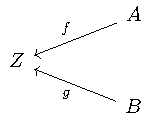
\includegraphics[height=2mm]{assets/images/Chapter_I/3.11a.pdf}}$ is a commutative diagram
        \[\begin{tikzcd}[row sep=0.8em,column sep=2em,ampersand replacement=\&]
            \&\&\& A \ar[dll, "f"] \ar[dlll, swap, bend right, "f"] \\
            Z \& Z \ar[l, swap, "\one_Z"] \\
            \&\&\& B \ar[ull, swap, "g"] \ar[ulll, bend left, "g"]
        \end{tikzcd}\]
        in $\cat{C}$. 
    \end{itemize}
    Then it can be immediately shown that $\cat{C}^{A,B}$ is a category.

    Secondly, we will fix two morphisms $\alpha : C \to A$, $\beta : C \to B$ where $A,B,C$ are fixed objects of $\cat{C}$. We can define a new category $\cat{C}^{\alpha,\beta}$ by essentially the same procedure that we used in order to define $\cat{C}^\alpha$:
    \begin{itemize}[label=$\bullet$]
        \item $\Obj{\cat{C}^{\alpha,\beta}}$ is the collection of all commutative diagrams
        \[\begin{tikzcd}[row sep=0.8em,column sep=2em,ampersand replacement=\&]
            \&\& A \ar[dll, swap, "f"] \\
            Z \&\&\&\& C \ar[dll, "\beta"] \ar[ull, swap, "\alpha"]\\
            \&\& B \ar[ull, "g"]
        \end{tikzcd}\]
        in $\cat{C}$;

        \item morphisms
        \[\begin{tikzcd}[row sep=0.8em,column sep=2em,ampersand replacement=\&]
            \&\& A \ar[dll, swap, "f_1"] \&\& \&\& \&\& A \ar[dll, swap, "f_2"]\\
            Z_1 \&\&\&\& C \ar[dll, "\beta"] \ar[ull, swap, "\alpha"] \ar[rr] \&\& Z_2 \&\&\&\& C \ar[dll, "\beta"] \ar[ull, swap, "\alpha"] \\
            \&\& B \ar[ull, "g_1"] \&\& \&\& \&\& B \ar[ull, "g_2"]
        \end{tikzcd}\]
        are commutative diagrams:
        \[\begin{tikzcd}[row sep=0.8em,column sep=2em,ampersand replacement=\&]
            \& \&\& A \ar[dll, swap, "f_2"] \ar[dlll, swap, bend right, "f_1"] \\
            Z_1 \& Z_2 \ar[l, "\sigma"] \&\&\&\& C \ar[dll, "\beta"] \ar[ull, swap, "\alpha"]\\
            \& \&\& B \ar[ull, "g_2"] \ar[ulll, bend left, "g_1"]
        \end{tikzcd}\]
        in $\cat{C}$;

        \item composition of two morphisms
        $$\begin{array}{ll}
            \begin{tikzcd}[row sep=0.8em,column sep=2em,ampersand replacement=\&]
                \& \&\& A \ar[dll, swap, "f_2"] \ar[dlll, swap, bend right, "f_1"] \\
                Z_1 \& Z_2 \ar[l, "\sigma"] \&\&\&\& C \ar[dll, "\beta"] \ar[ull, swap, "\alpha"]\\
                \& \&\& B \ar[ull, "g_2"] \ar[ulll, bend left, "g_1"]
            \end{tikzcd}, &
            \begin{tikzcd}[row sep=0.8em,column sep=2em,ampersand replacement=\&]
                \& \&\& A \ar[dll, swap, "f_3"] \ar[dlll, swap, bend right, "f_2"] \\
                Z_2 \& Z_3 \ar[l, "\tau"] \&\&\&\& C \ar[dll, "\beta"] \ar[ull, swap, "\alpha"]\\
                \& \&\& B \ar[ull, "g_3"] \ar[ulll, bend left, "g_2"]
            \end{tikzcd}
        \end{array}$$
        is a commutative diagram
        \[\begin{tikzcd}[row sep=0.8em,column sep=2em,ampersand replacement=\&]
            \& \&\& A \ar[dll, swap, "f_3"] \ar[dlll, swap, bend right, "f_1"] \\
            Z_1 \& Z_3 \ar[l, "\tau\sigma"] \&\&\&\& C \ar[dll, "\beta"] \ar[ull, swap, "\alpha"]\\
            \& \&\& B \ar[ull, "g_3"] \ar[ulll, bend left, "g_1"]
        \end{tikzcd}\]
        in $\cat{C}$; and

        \item an identity morphism $\one_{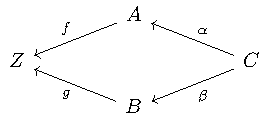
\includegraphics[height=2mm]{assets/images/Chapter_I/3.11b.pdf}}$ is a commutative diagram
        \[\begin{tikzcd}[row sep=0.8em,column sep=2em,ampersand replacement=\&]
            \& \&\& A \ar[dll, swap, "f"] \ar[dlll, swap, bend right, "f"] \\
            Z \& Z \ar[l, "\one_Z"] \&\&\&\& C \ar[dll, "\beta"] \ar[ull, swap, "\alpha"]\\
            \& \&\& B \ar[ull, "g"] \ar[ulll, bend left, "g"]
        \end{tikzcd}\]
        in $\cat{C}$.
    \end{itemize}
    Then it can be quite easily shown that $\cat{C}^{\alpha,\beta}$ is a category.
}